\section{Implementation} \label{implementation}

\subsection{Study Pipeline}

\begin{figure}[h]
\centering
    \subfigure[]{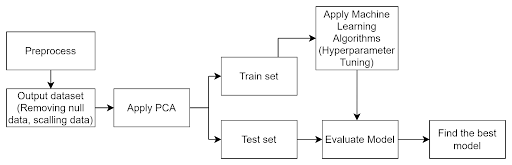
\includegraphics[width=1\textwidth]{image/framework.png}}
\caption{The models workflow} \label{fig:models-workflow}
\end{figure}

First of all, the data need to be prepared before applying with any model. 260 reflectance information files each including 2150 rows of figures. After proccessing the raw data and removing all the null data, the result is an output csv file with 168 row and 2154 collumns. The obtained data may contains features with a variety of dimensions and scales. These differences leads to a biased predictions results in terms of accuracy rates. To avoid this, it is necessary to implement standardization scale to the data before applying to modelin. The next step, the main works of this project, is the analysis and study the relationship of the reflectance data with the plants nutrients. The dataset is splitted into a train set and a test set with a 80-20 portions. To make the model more effective in exploring such a high-dimensional datasets, two methods is proposed. One is using PCA which have been widely used with machine learning algorithms. Others method, limiting which reflectance bandwidth is selected to ran through the models can show the correlation betwween the bandwidth and the plant's nutrient. Since multple models are used in this study, optuna is applied as a tool to automatically find the best hyperparameter for each corresponding models. Finally, the models is continously executed using the dataset that is limited by the red and infra-red bandwidth. From all the collected result, the prediction data and desirable wavelegth, we can conclude which one will be the best model and technique for resolving our challenge.  
 

\subsection{Tools \& Library}
For this project, most of the work is ran using ICTlab servers.
\begin{itemize}
    \item 
    Scikit-learn: Scikitlearn is an open-source machine learning library for Python. It offers several tools for various machine learning tasks including classification, regression, clustering, dimensional reduction, model selection, and data preprocessing. 
    \item 
    Optuna: This is an open-source hyperparameter optimization for machine learning models, which helps in finding the best hyperparameters, making it easier to improve performance and accuracy. Optuna contains various optimization algorithms to search for the optimal hyperparameter in a defined space.
    \item
    Numpy, Matplotlib: used for scientific computing and visualization. Numpy is used for numerical computing and Matplotlib is a tool for creating data visualization.
\end{itemize}

\subsection{Prepare the dataset}
As mentioned above, in this study, two type of dataset need to be put together. First is the main dataset which is the combination of 2 file. The csv file, which contain the measured data of the plant nutrients and its position. The sed file contain most of the information of the vegetation spectral reflectance, however it needs to filter a lot of noise data before merging.
Secondly, another dataset need to generated, the steps remain largely the same, except to analyse which bandwidth is most compatible, the spectral reflectance data need to be limited by the corresponding red and infra red bandwidth. While the highest bandwidth in the dataset is only 2500 nm, the number of time need to ran for each model is over 20000 combination. Most simple model can run through the experiements just fine, However for more advance model, this method could be quite taxing procedure.

\subsection{Hyperparameter Optimization}

Hyperparameter Optimization in Machine learning is the tool to select the best parameters for the learning algorithm. These hyperparameters find the values that can improve the efficiency of model performance. The main idea is to tune parameters to ensure that the model can handle data patterns and minimize a predefined loss function. Cross-validation is commonly used to estimate performance and choose the hyperparameter values that maximize it. There are several ways to optimize hyperparameters such as Grid Search, Random Search, etc. Grid Search is working when specifying a range of parameter values and testing them to see which will work best. This process requires performance metrics like cross-validation to guide the choice. However, when dealing with parameters that can take on real or unbounded values, we may need to set boundaries and discrete values before conducting the grid search. Grid Search is not such a great choice when working with high dimensional parameters space. So to work with more advance model likes AdaBoost, we choose Optuna\cite{optuna}, which is an automatic hyperparameter optimization framework, as a backup plan. Optuna runs based on the define-by-run approach, which will bring flexibility when working with high-dimensional spaces for hyperparameters. 

\subsection{Model Evaluation}

\subsubsection{Mean Squared Error (MSE)}
MSE quantifies the average squared difference between estimated values and actual values. In machine learning, it is one of the popular metrics when evaluating the quality of predictors or estimators. MSE is a non-negative value increasing as errors grow in the model. It considers both variance (how wide estimates vary across data samples) and bias (how far the average between estimates and true value). For an unbiased estimator, MSE equals the variance of the estimator. MSE can be given as the following equation:
\begin{quote}
    
    \(MSE = \frac{1}{n}\ \sum_{i=1}^{n}({\ Y}_{i} - {\widehat{Y}}_{i}\ )^2\)
\end{quote}

\begin{itemize}
    \item \(Y_{i}\): the i\_th observed value,
    \item \({\widehat{Y}}_{i}\): the corresponding predicted value,
    \item \(n\) = the number of observations.
\end{itemize}

\subsubsection{R square}
R squared or R2 (coefficient of determination) is one of the metrics to understand how the output values (variance of a dependent variable) are explained by an independent variable. The value ranges from 0 to 1 and can be negative if the model performs worse than the average fit. An R2 above 0.7 can be signified as a strong correlation, while below 0.4 signified a weaker one. 
\begin{quote}
    \(R^{2} = 1 - \frac{{SS}_{Regression}}{{SS}_{Total}}\)

\end{quote}
\begin{itemize}
    \item \({SS}_{Regression}\) : the sum of squares due to regression,
    \item \({SS}_{Total}\) : the total sum of squares.
\end{itemize}

\subsubsection{Mean Absolute Percentage Error (MAPE)}
Mean Absolute Percentage Error (MAPE) is a metric for evaluating the accuracy of predicting methods, especially when we are working with large and nonzero dataset values. It calculates the percentage error between predicted and actual values. A MAPE below 5\% is a highly accurate prediction, while a MAPE between 10\% and 25\% is acceptable. But when it exceeds 25\%, it means that the results come out have very low accuracy, equivalent to an unacceptable prediction. 

\begin{quote}
    
    \(MAPE = \frac{1}{n} \sum_{t=1}^{n}\left| \frac{A_{t} - F_{t}}{A_{t}} \right|\)
\end{quote}
\begin{itemize}
    \item  \(n\) : sample size,
    \item  \(A_{t}\): the actual data value,
    \item  \(F_{t}\): the forecasted data value.
\end{itemize}